\documentclass[12pt]{article}
\usepackage[english]{babel}
\usepackage[utf8x]{inputenc}
\usepackage{amsmath}
\usepackage{tikz}
\usetikzlibrary{arrows,automata}
\begin{document}

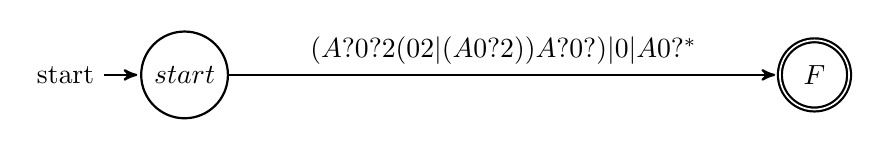
\begin{tikzpicture}[->,>=stealth',shorten >=1pt,auto,node distance=8cm,
    thick,base node/.style={circle,draw,minimum size=8pt}, real node/.style={double,circle,draw,minimum size=17pt}]

  \node[state,initial] (start) {$start$};
 
  \node[state,accepting] (F) [right of=start] {$F$};
  
  \path 
        (start) edge   node {$(A?0?2(02|(A0?2))A?0?)|0|A0?^{*}$}(F);
       
        
\end{tikzpicture}
        $$A=0?1(01)^{*}$$
\end{document}https://www.overleaf.com/project/5f66c6dd8387d300018234e8